\section{Counting bits set to 1}

Here is a simple example of a function that calculates the number of bits set in the input value.

This operation is also called \q{population count}\footnote{modern x86 CPUs (supporting SSE4) even have a POPCNT instruction for it}.

\lstinputlisting{patterns/14_bitfields/4_popcnt/shifts.c}

In this loop, the iteration count value $i$ is counting from 0 to 31, 
so the $1 \ll i$ statement is counting from 1 to \TT{0x80000000}.
Describing this operation in natural language, we would say \IT{shift 1 by n bits left}.
In other words, $1 \ll i$ statement consequently produces all possible bit positions in a 32-bit number.
The freed bit at right is always cleared.

Here is a table of all possible $1 \ll i$ 
for $i=0 \ldots 31$:

\begin{center}
\begin{tabular}{ | l | l | l | l | }
\hline
\HeaderColor \CCpp expression & 
\HeaderColor Power of two & 
\HeaderColor Decimal form & 
\HeaderColor Hexadecimal form \\
\hline
$1 \ll 0$ & 1 & 1 & 1 \\
\hline
$1 \ll 1$ & $2^{1}$ & 2 & 2 \\
\hline
$1 \ll 2$ & $2^{2}$ & 4 & 4 \\
\hline
$1 \ll 3$ & $2^{3}$ & 8 & 8 \\
\hline
$1 \ll 4$ & $2^{4}$ & 16 & 0x10 \\
\hline
$1 \ll 5$ & $2^{5}$ & 32 & 0x20 \\
\hline
$1 \ll 6$ & $2^{6}$ & 64 & 0x40 \\
\hline
$1 \ll 7$ & $2^{7}$ & 128 & 0x80 \\
\hline
$1 \ll 8$ & $2^{8}$ & 256 & 0x100 \\
\hline
$1 \ll 9$ & $2^{9}$ & 512 & 0x200 \\
\hline
$1 \ll 10$ & $2^{10}$ & 1024 & 0x400 \\
\hline
$1 \ll 11$ & $2^{11}$ & 2048 & 0x800 \\
\hline
$1 \ll 12$ & $2^{12}$ & 4096 & 0x1000 \\
\hline
$1 \ll 13$ & $2^{13}$ & 8192 & 0x2000 \\
\hline
$1 \ll 14$ & $2^{14}$ & 16384 & 0x4000 \\
\hline
$1 \ll 15$ & $2^{15}$ & 32768 & 0x8000 \\
\hline
$1 \ll 16$ & $2^{16}$ & 65536 & 0x10000 \\
\hline
$1 \ll 17$ & $2^{17}$ & 131072 & 0x20000 \\
\hline
$1 \ll 18$ & $2^{18}$ & 262144 & 0x40000 \\
\hline
$1 \ll 19$ & $2^{19}$ & 524288 & 0x80000 \\
\hline
$1 \ll 20$ & $2^{20}$ & 1048576 & 0x100000 \\
\hline
$1 \ll 21$ & $2^{21}$ & 2097152 & 0x200000 \\
\hline
$1 \ll 22$ & $2^{22}$ & 4194304 & 0x400000 \\
\hline
$1 \ll 23$ & $2^{23}$ & 8388608 & 0x800000 \\
\hline
$1 \ll 24$ & $2^{24}$ & 16777216 & 0x1000000 \\
\hline
$1 \ll 25$ & $2^{25}$ & 33554432 & 0x2000000 \\
\hline
$1 \ll 26$ & $2^{26}$ & 67108864 & 0x4000000 \\
\hline
$1 \ll 27$ & $2^{27}$ & 134217728 & 0x8000000 \\
\hline
$1 \ll 28$ & $2^{28}$ & 268435456 & 0x10000000 \\
\hline
$1 \ll 29$ & $2^{29}$ & 536870912 & 0x20000000 \\
\hline
$1 \ll 30$ & $2^{30}$ & 1073741824 & 0x40000000 \\
\hline
$1 \ll 31$ & $2^{31}$ & 2147483648 & 0x80000000 \\
\hline
\end{tabular}
\end{center}

These constant numbers (bit masks) very often appear in code and a practicing reverse engineer 
must be able to spot them quickly.

You probably haven't to memorize the decimal numbers, but the hexadecimal ones are very easy to remember.

These constants are very often used for mapping flags to specific bits.
For example, here is excerpt from \TT{ssl\_private.h} 
from Apache 2.4.6 source code:

\begin{lstlisting}
/**
 * Define the SSL options
 */
#define SSL_OPT_NONE           (0)
#define SSL_OPT_RELSET         (1<<0)
#define SSL_OPT_STDENVVARS     (1<<1)
#define SSL_OPT_EXPORTCERTDATA (1<<3)
#define SSL_OPT_FAKEBASICAUTH  (1<<4)
#define SSL_OPT_STRICTREQUIRE  (1<<5)
#define SSL_OPT_OPTRENEGOTIATE (1<<6)
#define SSL_OPT_LEGACYDNFORMAT (1<<7)
\end{lstlisting}

Let's get back to our example.

The \TT{IS\_SET} macro checks bit presence in $a$.
\myindex{x86!\Instructions!AND}

The \TT{IS\_SET} macro is in fact the logical AND operation (\IT{AND}) 
and it returns 0 if the specific bit is absent there,
or the bit mask, if the bit is present.
\IT{The if()} operator in \CCpp triggers if the expression in it is not zero, it might be even 123456, that is why
it always works correctly.

% subsections
\subsection{x86}

\subsubsection{MSVC}

Let's compile (MSVC 2010):

\lstinputlisting[caption=MSVC 2010]{patterns/14_bitfields/4_popcnt/shifts_MSVC_EN.asm}

\clearpage
\myparagraphold{\olly}
\myindex{\olly}

Let's load this example into \olly. 
Let the input value be \TT{0x12345678}.

For $i=1$, we see how $i$ is loaded into \ECX: 

\begin{figure}[H]
\centering
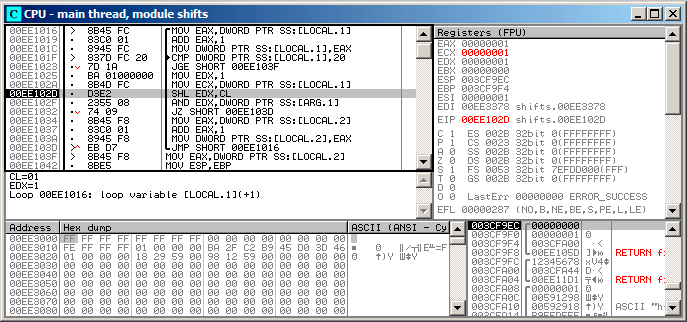
\includegraphics[scale=\FigScale]{patterns/14_bitfields/4_popcnt/olly1_1.png}
\caption{\olly: $i=1$, $i$ is loaded into \ECX}
\label{fig:shifts_olly1_1}
\end{figure}

\EDX is 1. \SHL is to be executed now.

\clearpage
\SHL was executed:

\begin{figure}[H]
\centering
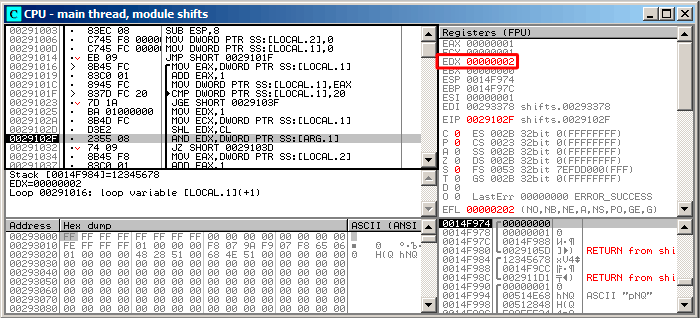
\includegraphics[scale=\FigScale]{patterns/14_bitfields/4_popcnt/olly1_2.png}
\caption{\olly: $i=1$, \EDX=$1 \ll 1=2$}
\label{fig:shifts_olly1_2}
\end{figure}

\EDX contain $1 \ll 1$ (or 2). This is a bit mask.

\clearpage
\AND sets \ZF to 1, which implies that the input value (\TT{0x12345678})  ANDed with 2 results in 0:

\begin{figure}[H]
\centering
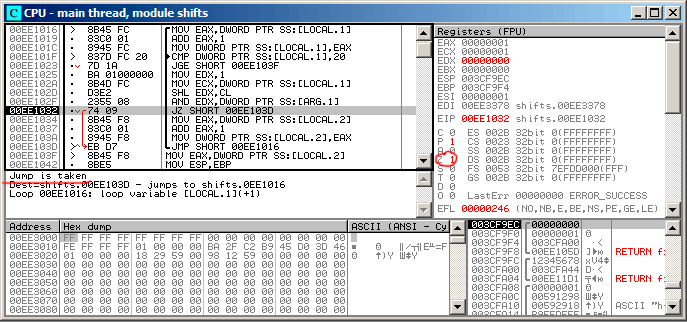
\includegraphics[scale=\FigScale]{patterns/14_bitfields/4_popcnt/olly1_3.png}
\caption{\olly: $i=1$, 
is there that bit in the input value? No. (\ZF=1)}
\label{fig:shifts_olly1_3}
\end{figure}

So, there is no corresponding bit in the input value.

The piece of code, which \glslink{increment}{increments} the counter is not to be executed: 
the \JZ instruction \emph{bypassing} it.

\clearpage
Let's trace a bit further and $i$ is now 4.
\SHL is to be executed now:

\begin{figure}[H]
\centering
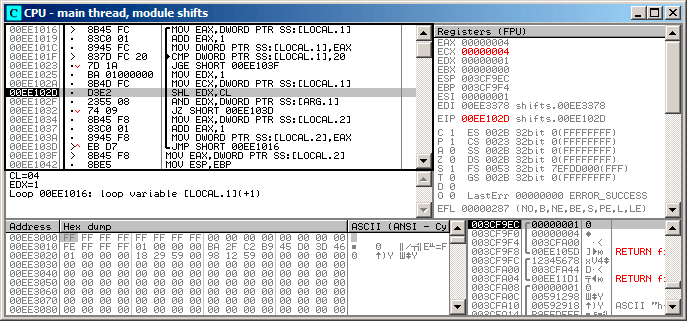
\includegraphics[scale=\FigScale]{patterns/14_bitfields/4_popcnt/olly4_1.png}
\caption{\olly: $i=4$, $i$ is loaded into \ECX}
\label{fig:shifts_olly4_1}
\end{figure}

\clearpage
\EDX=$1 \ll 4$ (or \TT{0x10} or 16): 

\begin{figure}[H]
\centering
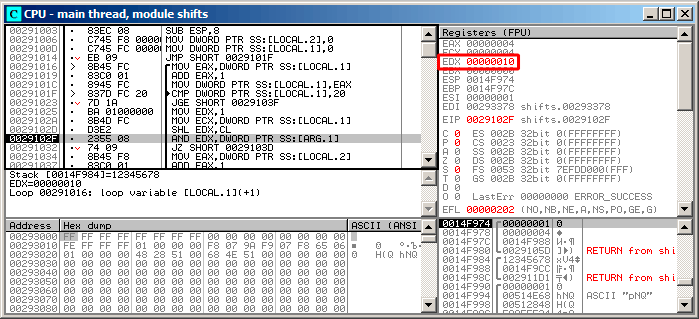
\includegraphics[scale=\FigScale]{patterns/14_bitfields/4_popcnt/olly4_2.png}
\caption{\olly: $i=4$, \EDX=$1 \ll 4=0x10$}
\label{fig:shifts_olly4_2}
\end{figure}

This is another bit mask.

\clearpage
\AND is executed:

\begin{figure}[H]
\centering
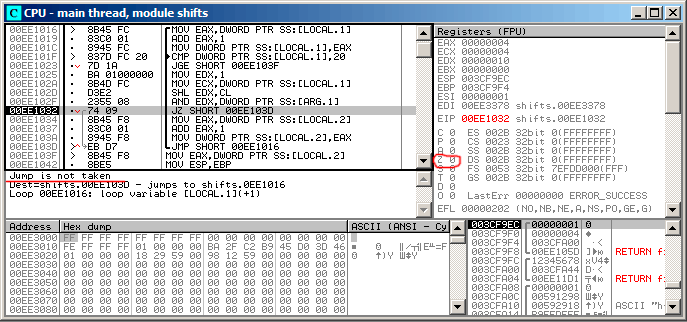
\includegraphics[scale=\FigScale]{patterns/14_bitfields/4_popcnt/olly4_3.png}
\caption{\olly: $i=4$, 
is there that bit in the input value? Yes. (\ZF=0)}
\label{fig:shifts_olly4_3}
\end{figure}

\ZF is 0 because this bit is present in the input value.
Indeed, \TT{0x12345678 \& 0x10 = 0x10}. 

This bit counts: the jump is not triggering and the bit counter 
\glslink{increment}{incrementing}.

The function returns 13. 
This is total number of bits set in \TT{0x12345678}.



\subsubsection{GCC}

Let's compile it in GCC 4.4.1:

\lstinputlisting[caption=GCC 4.4.1]{patterns/14_bitfields/4_popcnt/shifts_gcc.asm}

\subsection{x64}
\label{subsec:popcnt}

Let's modify the example slightly to extend it to 64-bit:

\lstinputlisting[label=popcnt_x64_example]{patterns/14_bitfields/4_popcnt/shifts64.c}

\subsubsection{\NonOptimizing GCC 4.8.2}

So far so easy.

\lstinputlisting[caption=\NonOptimizing GCC 4.8.2]{patterns/14_bitfields/4_popcnt/shifts64_GCC_O0_EN.s}

\subsubsection{\Optimizing GCC 4.8.2}

\lstinputlisting[caption=\Optimizing GCC 4.8.2,numbers=left,label=shifts64_GCC_O3]{patterns/14_bitfields/4_popcnt/shifts64_GCC_O3_EN.s}

This code is terser, but has a quirk.

In all examples that we see so far, we were incrementing the \q{rt} value after comparing a specific bit,
but the code here increments \q{rt} before (line 6), writing the new value into register \EDX .
Thus, if the last bit is 1, the \CMOVNE\footnote{Conditional MOVe if Not Equal} instruction
(which is a synonym for \CMOVNZ\footnote{Conditional MOVe if Not Zero}) \IT{commits} 
the new value of \q{rt}
by moving \EDX (\q{proposed rt value}) into \EAX (\q{current rt} to be returned at the end).

Hence, the incrementing is done at each step of loop, i.e., 64 times, without any relation to the input value.

The advantage of this code is that it contain only one conditional jump (at the end of the loop) instead of 
two jumps (skipping the \q{rt} value increment and at the end of loop).
And that might work faster on the modern CPUs with branch predictors: \myref{branch_predictors}.

\label{FATRET}
\myindex{x86!\Instructions!FATRET}
The last instruction is \INS{REP RET} (opcode \TT{F3 C3}) 
which is also called \INS{FATRET} by MSVC.
This is somewhat optimized version of \RET, 
which is recommended by AMD to be placed at the end of function, if \RET goes right after conditional jump: 
[\AMDOptimization p.15]
\footnote{More information on it: \url{http://go.yurichev.com/17328}}.

\subsubsection{\Optimizing MSVC 2010}

\lstinputlisting[caption=MSVC 2010]{patterns/14_bitfields/4_popcnt/MSVC_2010_x64_Ox_EN.asm}

\myindex{x86!\Instructions!ROL}
Here the \ROL instruction is used instead of 
\SHL, which is in fact \q{rotate left} 
instead of \q{shift left},
but in this example it works just as \TT{SHL}.

You can read more about the rotate instruction here: \myref{ROL_ROR}.

\Reg{8} here is counting from 64 to 0.
It's just like an inverted $i$.

Here is a table of some registers during the execution:

\begin{center}
\begin{tabular}{ | l | l | }
\hline
\HeaderColor RDX & \HeaderColor R8 \\
\hline
0x0000000000000001 & 64 \\
\hline
0x0000000000000002 & 63 \\
\hline
0x0000000000000004 & 62 \\
\hline
0x0000000000000008 & 61 \\
\hline
... & ... \\
\hline
0x4000000000000000 & 2 \\
\hline
0x8000000000000000 & 1 \\
\hline
\end{tabular}
\end{center}

\myindex{x86!\Instructions!FATRET}
At the end we see the \INS{FATRET} instruction, which was explained here: \myref{FATRET}.

\subsubsection{\Optimizing MSVC 2012}

\lstinputlisting[caption=MSVC 2012]{patterns/14_bitfields/4_popcnt/MSVC_2012_x64_Ox_EN.asm}

\myindex{\CompilerAnomaly}
\label{MSVC2012_anomaly}
\Optimizing MSVC 2012 does almost the same job as 
optimizing MSVC 2010, but somehow, it generates two identical loop bodies and the loop count is now 32 instead of 64.

To be honest, it's not possible to say why. Some optimization trick? Maybe it's better for the loop body to be slightly 
longer?

Anyway, such code is relevant here to show that sometimes the compiler output may be really weird and 
illogical, but perfectly working.


\subsubsection{ARM + \OptimizingXcodeIV (\ARMMode)}

\lstinputlisting[caption=\OptimizingXcodeIV (\ARMMode),label=ARM_leaf_example4]{patterns/14_bitfields/4_popcnt/ARM_Xcode_O3_EN.lst}

\myindex{ARM!\Instructions!TST}
\TST is the same things as \TEST in x86.

\myindex{ARM!Optional operators!LSL}
\myindex{ARM!Optional operators!LSR}
\myindex{ARM!Optional operators!ASR}
\myindex{ARM!Optional operators!ROR}
\myindex{ARM!Optional operators!RRX}
\myindex{ARM!\Instructions!MOV}
\myindex{ARM!\Instructions!TST}
\myindex{ARM!\Instructions!CMP}
\myindex{ARM!\Instructions!ADD}
\myindex{ARM!\Instructions!SUB}
\myindex{ARM!\Instructions!RSB}
As was noted before~(\myref{shifts_in_ARM_mode}),
there are no separate shifting instructions in ARM mode.
However, there are modifiers 
LSL (\IT{Logical Shift Left}), 
LSR (\IT{Logical Shift Right}), 
ASR (\IT{Arithmetic Shift Right}), 
ROR (\IT{Rotate Right}) and
RRX (\IT{Rotate Right with Extend}), which may be added to such instructions as \MOV, \TST,
\CMP, \ADD, \SUB, \RSB\footnote{\DataProcessingInstructionsFootNote}.

These modificators define how to shift the second operand and by how many bits.

\myindex{ARM!\Instructions!TST}
\myindex{ARM!Optional operators!LSL}
Thus the \TT{\q{TST R1, R2,LSL R3}} instruction works here as $R1 \land (R2 \ll R3)$.

\subsubsection{ARM + \OptimizingXcodeIV (\ThumbTwoMode)}

\myindex{ARM!\Instructions!LSL.W}
\myindex{ARM!\Instructions!LSL}
Almost the same, but here are two \INS{LSL.W}/\TST instructions are used instead of a single \TST, because in Thumb mode it is not
possible to define \LSL modifier directly in \TST.

\begin{lstlisting}[label=ARM_leaf_example5]
                MOV             R1, R0
                MOVS            R0, #0
                MOV.W           R9, #1
                MOVS            R3, #0
loc_2F7A
                LSL.W           R2, R9, R3
                TST             R2, R1
                ADD.W           R3, R3, #1
                IT NE
                ADDNE           R0, #1
                CMP             R3, #32
                BNE             loc_2F7A
                BX              LR
\end{lstlisting}

\subsubsection{ARM64 + \Optimizing GCC 4.9}

Let's take the 64-bit example which has been already used: \myref{popcnt_x64_example}.

\lstinputlisting[caption=\Optimizing GCC (Linaro) 4.8]{patterns/14_bitfields/4_popcnt/ARM64_GCC_O3_EN.s}

The result is very similar to what GCC generates for x64: \myref{shifts64_GCC_O3}.

\myindex{ARM!\Instructions!CSEL}
The \CSEL instruction is \q{Conditional SELect}. 
It just chooses one variable of two depending on the flags set by \TST and copies the value into \RegW{2}, which holds the \q{rt} variable.

\subsubsection{ARM64 + \NonOptimizing GCC 4.9}

And again, we'll work on the 64-bit example which was already used: \myref{popcnt_x64_example}.
The code is more verbose, as usual.

\lstinputlisting[caption=\NonOptimizing GCC (Linaro) 4.8]{patterns/14_bitfields/4_popcnt/ARM64_GCC_O0_EN.s}


\subsection{MIPS}

\subsubsection{\NonOptimizing GCC}

\lstinputlisting[caption=\NonOptimizing GCC 4.4.5 (IDA)]{patterns/14_bitfields/4_popcnt/MIPS_O0_IDA_EN.lst}

\myindex{MIPS!\Instructions!SLL}
\myindex{MIPS!\Instructions!SLLV}

That is verbose: all local variables are located in the local stack and reloaded each time they're needed.

The \SLLV instruction is \q{Shift Word Left Logical Variable}, it differs from \SLL only in that
the shift amount is encoded in the \SLL instruction (and is fixed, as a consequence), 
but \SLLV takes shift amount from a register.

\subsubsection{\Optimizing GCC}

That is terser.
There are two shift instructions instead of one.
Why?

It's possible to replace the first \SLLV instruction with an unconditional branch instruction that jumps right to the second \SLLV.
But this is another branching instruction in the function, and it's always favorable to get rid of them: \myref{branch_predictors}.

\lstinputlisting[caption=\Optimizing GCC 4.4.5 (IDA)]{patterns/14_bitfields/4_popcnt/MIPS_O3_IDA_EN.lst}


